\begin{frame}
    \begin{center}
        \small
        Волгоградский Государственный Технический Университет \\
        Факультет электроники и вычислительной техники \\
        Кафедра физики \\
        \vspace{1.5cm}
        Выпускная работа на тему: \\
        \normalsize
        \textbf{Моделирование структуры абрикосовских вихрей в 
            сверхпроводниках типа 1,5} \\
        \vspace{1.5cm}
        \small
        Автор работы --- студент Ф-469 Голубев А. В. \\
        Научный руководитель --- д.ф.--м.н. Завьялов Д. В. \\
        \vspace{\fill}
        Волгоград \the\year
    \end{center}
\end{frame}

\begin{frame}
    \frametitle{Цель}
    \begin{itemize}
        \item исследование появления сверхпроводимости типа 1,5;
        \item исследования случая многополосной сверхпроводимости;
        \item теоретический анализ модели;
        \item моделирование структуры абрикосовских вихрей;
    \end{itemize}
\end{frame}

\begin{frame}
    \frametitle{Актуальность работы}
    \begin{itemize}
        \item широкие возможностями применения сверхпроводников в 
            современной микроэлектронике;
        \item высокотемпературные сверхпроводники;
        \item малая изученность физики данного процесса;
        \item перспективность в исследовании смешанного состояния;
    \end{itemize}
\end{frame}

\begin{frame}
    \frametitle{Фазовая диаграмма}
    \begin{figure}[h]
        \center
        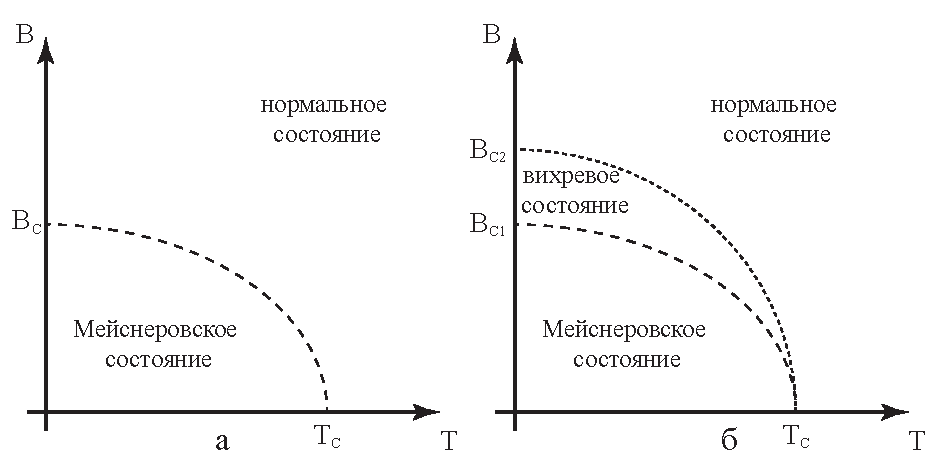
\includegraphics[width=1.0\linewidth]{img_01}
        \caption{Фазовая диаграмма состояния сверхпроводников 1-го (а) и 
            2-го (б) рода}
    \end{figure}
\end{frame}

\begin{frame}
    \frametitle{Фазовая диаграмма магнитных фаз}
    \begin{figure}[h]
        \center
        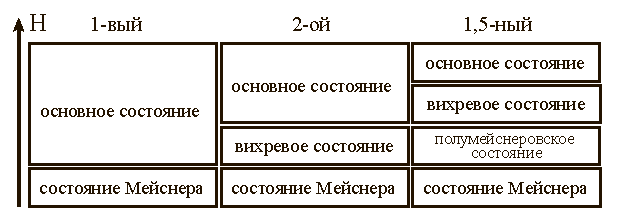
\includegraphics[width=1.0\linewidth]{1-02}
        \caption{Сравнение фазовых диаграмм магнитных фаз чистых 
            сверхпроводников первого, второго и полуторного рода при нулевой 
            температуре.}
    \end{figure}
\end{frame}

\begin{frame}
    \frametitle{Двухкомпонентная модель Гинзбурга-Ландау}
    \begin{gather}
        F = \frac{1}{2}(D\psi_1)(D\psi_1)^* + 
            \frac{1}{2}(D\psi_2)(D\psi_2)^* - \nonumber \\ -
            \nu Re\left( (D\psi_1)(D\psi_2)^* \right) +
            \frac{1}{2}\left(\nabla\times\vec{A}\right)^2 + F_p
    \end{gather}
    Здесь \( D = \nabla + ie\vec{A} \) и \( \psi_a = |\psi_a|e^{i\theta_a} \), 
    \( a = 1,2 \).
\end{frame}

\begin{frame}
    \frametitle{Метод моделирование структуры вихрей}
    \framesubtitle{}
\end{frame}

\begin{frame}
    \frametitle{Результаты модельного эксперимента}
    \framesubtitle{Поперечное сечение вихрей}
    \begin{figure}[h]
        \center
        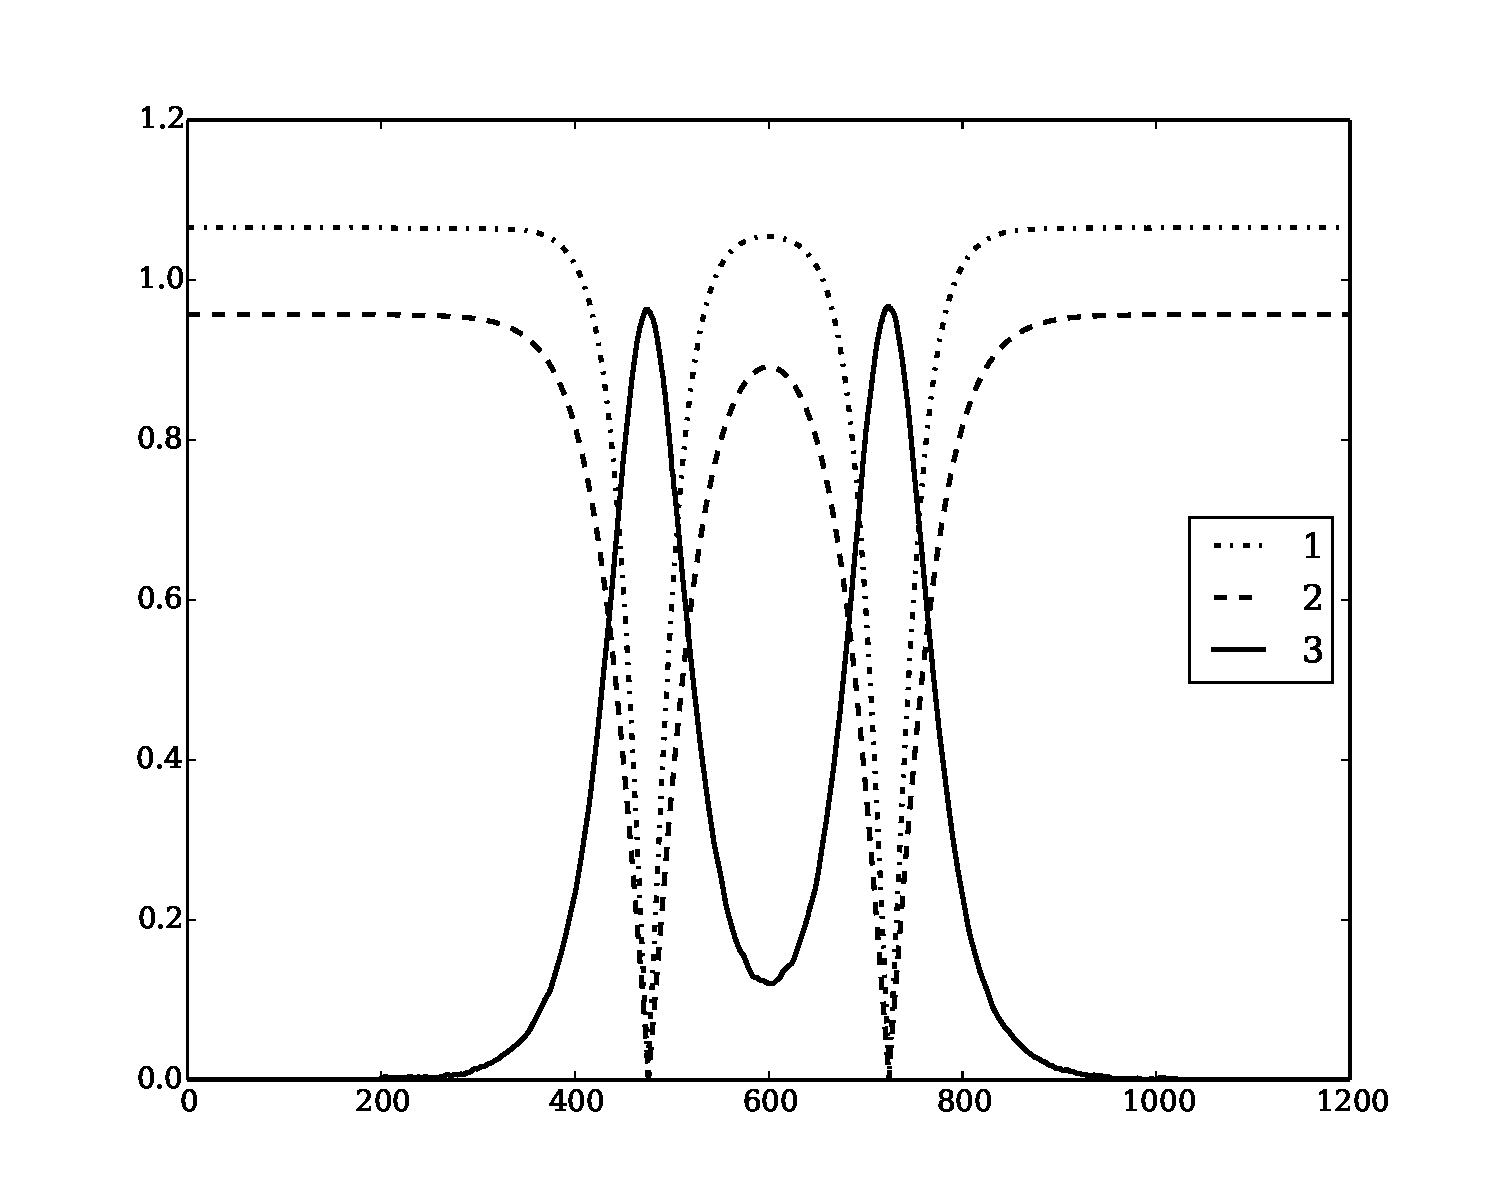
\includegraphics[width=0.8\linewidth]{band_profile}
    \end{figure}
\end{frame}

\begin{frame}
    \frametitle{Результаты модельного эксперимента}
    \framesubtitle{Распределение магнитного поля (\( B \))}
    \begin{figure}[h]
        \begin{minipage}[h]{0.49\linewidth}
            \center{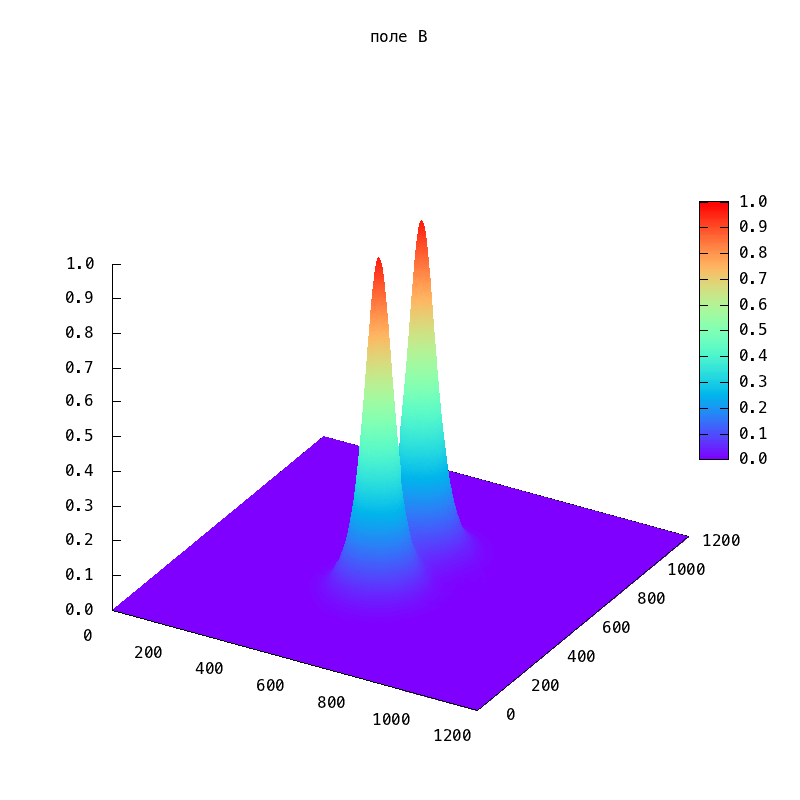
\includegraphics[width=1.1\linewidth]{3d_B}}
        \end{minipage}
        \hfill
        \begin{minipage}[h]{0.49\linewidth}
            \center{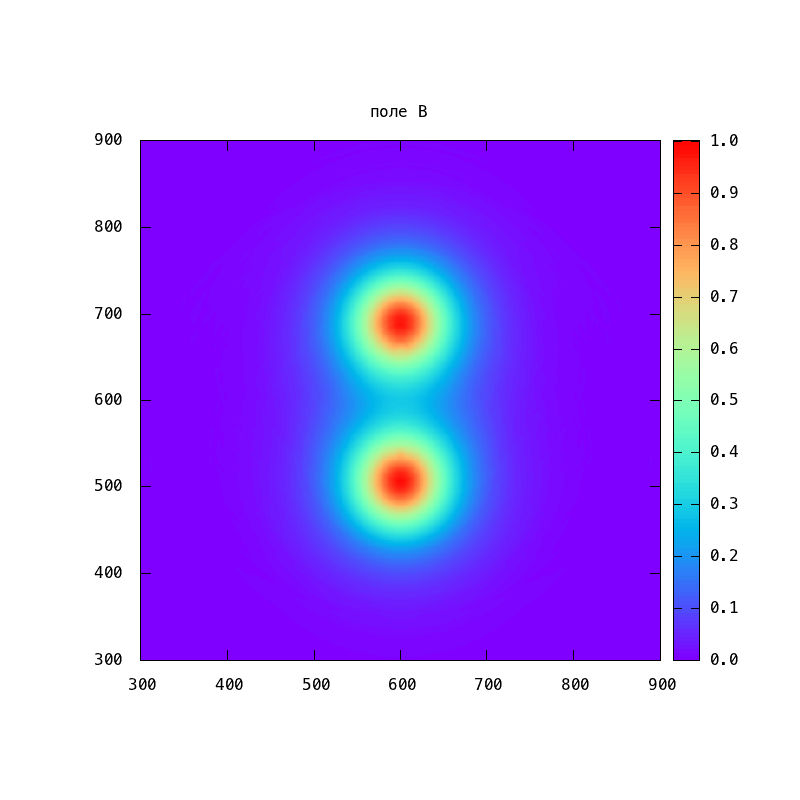
\includegraphics[width=1.1\linewidth]{map_B}}
        \end{minipage}
    \end{figure}
\end{frame}

\begin{frame}
    \frametitle{Результаты модельного эксперимента}
    \framesubtitle{Характерный вид энергии взаимодействия первой зоны в 
        сверхпроводнике (\( \abs{\psi_1}^2 \)-компонента).}
    \begin{figure}[h]
        \begin{minipage}[h]{0.49\linewidth}
            \center{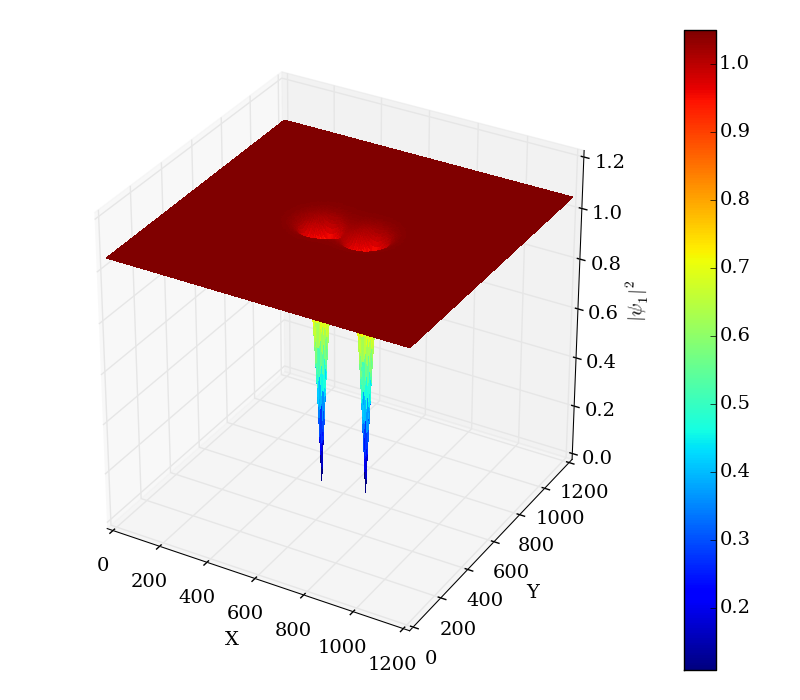
\includegraphics[width=1.1\linewidth]{3d_F1}}
        \end{minipage}
        \hfill
        \begin{minipage}[h]{0.49\linewidth}
            \center{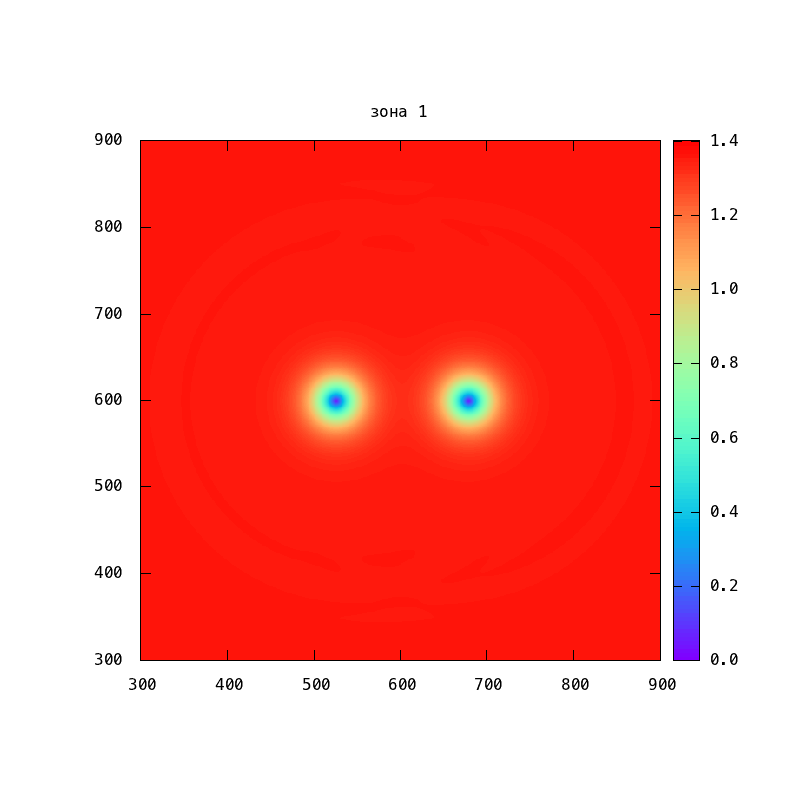
\includegraphics[width=1.1\linewidth]{map_F1}}
        \end{minipage}
    \end{figure}
\end{frame}

\begin{frame}
    \frametitle{Результаты модельного эксперимента}
    \framesubtitle{Характерный вид энергии взаимодействия первой зоны в 
        сверхпроводнике (\( \abs{\psi_2}^2 \)-компонента).}
    \begin{figure}[h]
        \begin{minipage}[h]{0.49\linewidth}
            \center{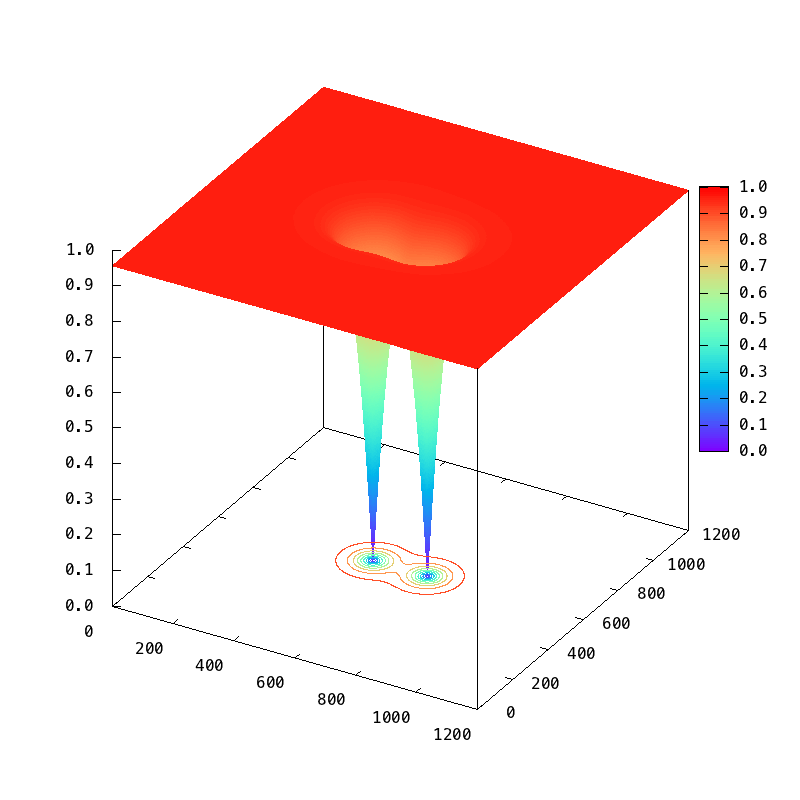
\includegraphics[width=1.1\linewidth]{3d_F2}}
        \end{minipage}
        \hfill
        \begin{minipage}[h]{0.49\linewidth}
            \center{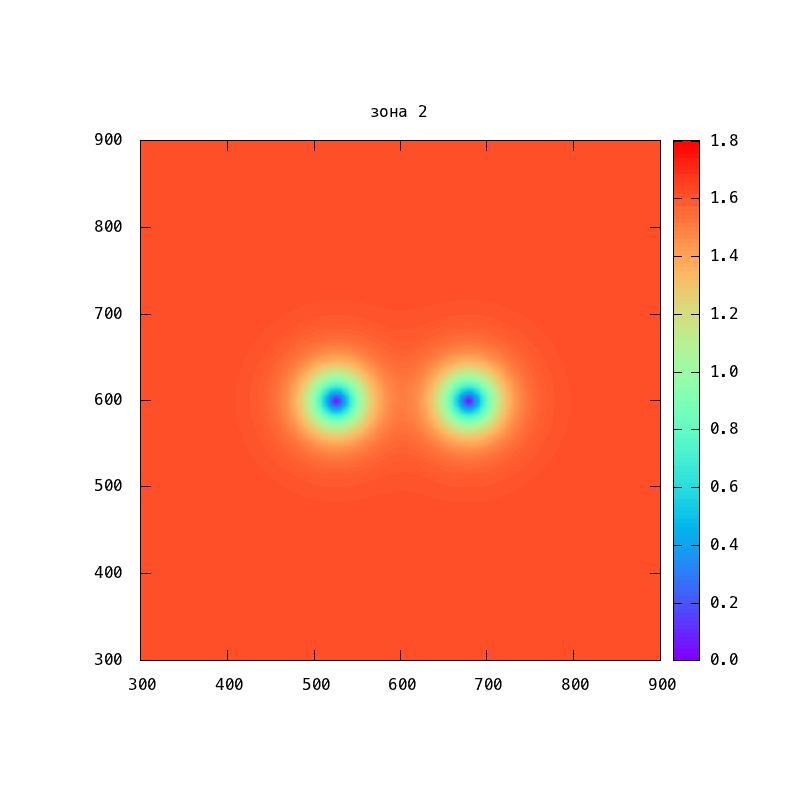
\includegraphics[width=1.1\linewidth]{map_F2}}
        \end{minipage}
    \end{figure}
\end{frame}